\documentclass[11pt]{article}

\usepackage[utf8]{inputenc}
\usepackage[T1]{fontenc}
\usepackage{lmodern}
\usepackage[margin=1in]{geometry}
\usepackage{microtype}
\usepackage{amsmath,amssymb}
\usepackage{booktabs}
\usepackage{multirow}
\usepackage{graphicx}
\usepackage{caption}
\usepackage{enumitem}
\usepackage{xurl}
\usepackage[colorlinks=true,linkcolor=blue,urlcolor=blue,citecolor=blue]{hyperref}
\usepackage[style=nature,backend=biber,maxbibnames=1,minbibnames=1,doi=false,url=false,isbn=false]{biblatex}
\addbibresource{references.bib}

\graphicspath{{figures/}{../figures/}}
\captionsetup{font=small,labelfont=bf}
\setlength{\parindent}{0pt}
\setlength{\parskip}{4pt}
\setlist[itemize]{leftmargin=*, itemsep=1pt, topsep=2pt}

\makeatletter
\renewcommand\section{\@startsection{section}{1}{\z@}%
    {-1.6ex \@plus -.5ex \@minus -.2ex}{0.7ex \@plus .2ex}%
    {\normalfont\large\bfseries}}
\makeatother

\usepackage{titling}
\setlength{\droptitle}{-4em}
\title{\Large\bfseries Distilling Compact Gene Panels for Retinal Cell-Type Annotation:\\ Interim Report}
\author{Luana Liao (\href{mailto:ll3637@columbia.edu}{ll3637@columbia.edu}) \and
        Sky Sun (\href{mailto:ms6124@columbia.edu}{ms6124@columbia.edu})}
\date{November 2026}

\begin{document}
\maketitle
\vspace{-1.5em}

% ---------------------------------------------------------------------------
\section{Introduction}

Targeted spatial transcriptomics measures only a few dozen to a few hundred genes per
experiment, so the gene panel must be chosen in advance. We ask \emph{how small a gene
panel can reliably identify human retinal cell types across donors and laboratories}, and
whether the selected genes match known markers and are supported by cell-type-specific
chromatin accessibility.

We train on the Human Retina Cell Atlas (HRCA; 3.2M single-nucleus transcriptomes from 104
donors~\cite{li2026}) and test without retraining on an independent multiome dataset from
another lab~\cite{wang2022}. That dataset's paired ATAC-seq lets us check the selected genes
against chromatin accessibility. Our method is a concrete (Gumbel-softmax) gene
selector~\cite{abid2019,jang2017} that restricts a classifier to exactly $k$ genes. It can
also include a donor-adversarial head trained with gradient reversal~\cite{ganin2016}, which
discourages donor-specific genes. We follow the course feedback in three ways. We compare
against simple panels of the same size: Wilcoxon differentially expressed (DE) genes, top
highly variable genes (HVG), and random genes. We add harder subtype tasks for bipolar (BC),
retinal ganglion (RGC) and amacrine (AC) cells. And we will test the ATAC support of learned
panels against DE panels of the same size, rather than only against random genes. Later
comparisons are PERSIST~\cite{covert2023}, frozen TranscriptFormer
embeddings~\cite{pearce2025}, and Pan-human Azimuth~\cite{azimuth2026}.

% ---------------------------------------------------------------------------
\section{Data}

\textbf{Sources.} Both datasets were downloaded as h5ad files from CZ
CELLxGENE~\cite{cellxgene2025}. The HRCA ``all cells'' snRNA-seq file is 37.7\,GB and holds
3{,}177{,}310 nuclei from 104 donors. They come from six studies in two labs: Chen lab
(Baylor, 87 donors) and Shekhar lab (Harvard, 17 donors). Fine subtype labels live in
separate HRCA BC/AC/RGC files. We fetched only their metadata over HTTP and joined it on the
shared cell identifier, which avoids downloading another 21\,GB. The Wang et
al.~\cite{wang2022} file has 51{,}645 multiome nuclei from 4 donors. It stores only
$\log(1+\mathrm{CP10k})$ values, so we recovered integer counts exactly: we inverted the
transform and divided each cell by its smallest nonzero value (maximum rounding error
$6\times10^{-4}$). For ATAC we downloaded the authors' per-cell-type fragment files (13 cell
types, 8\,GB, GEO GSE196235).

\textbf{Preprocessing.} We map Cell Ontology labels to 9 major classes shared by both
datasets: rod, cone, BC, AC, horizontal cell (HC), RGC, M\"uller glia (MG), astrocyte and
microglia. We drop retinal pigment epithelium (863 contaminating cells). We keep cells with
at least 300 detected genes and at most 10\% mitochondrial reads, and remove doublets with
Scrublet~\cite{wolock2019} run per donor. Only 0.1\% of HRCA cells and 0.03\% of Wang cells
were flagged, consistent with the authors' own filtering. Genes are the 35{,}449 Ensembl IDs
shared by both datasets. The two datasets share no donors, since HRCA's snRNA-seq comes only
from the Chen and Shekhar labs. To make the class distribution even, we capped the major
task at 400 cells per (donor, class). For subtypes we capped at 60 cells per (donor,
subtype) and kept subtypes with at least 300 cells in the atlas. Table~\ref{tab:data}
summarizes the result.

\begin{table}[h]
\centering\small
\caption{Datasets after QC. Median genes and UMIs are per cell.}
\label{tab:data}
\begin{tabular}{lrrrrr}
\toprule
 & cells & donors & classes & median genes & median UMIs \\
\midrule
HRCA major-class task & 272{,}687 & 104 & 9 & \multirow{4}{*}{2{,}671} & \multirow{4}{*}{5{,}592} \\
HRCA BC subtypes & 68{,}700 & 104 & 14 & & \\
HRCA RGC subtypes & 20{,}080 & 101 & 10 & & \\
HRCA AC subtypes & 185{,}778 & 104 & 71 & & \\
Wang 2022 (external test) & 51{,}504 & 4 & 9 & 1{,}425 & 2{,}649 \\
\bottomrule
\end{tabular}
\end{table}

\textbf{Exploratory analysis.} The atlas is dominated by rods (34\% of nuclei), and the
classes are very imbalanced: 1.07M rods vs.\ 4.9k microglia. Wang is even more skewed, with
62\% rods and only 231 microglia. Subtypes are imbalanced too. Midget cells make up 95\% of
RGCs, and many RGC types have fewer than 300 nuclei, so only 10 of 21 RGC types qualify for
the task. Wang nuclei have about half the depth of HRCA nuclei (Table~\ref{tab:data}), which
adds an assay shift on top of the lab shift.

Fig.~\ref{fig:pca}a shows PCA on 3{,}000 seurat-v3 HVGs~\cite{stuart2019}, using HRCA cells
from the major task plus 20k Wang cells. Cell classes separate clearly. PCs~1--2 split
photoreceptors, inner-retinal neurons and glia into three arms. MG and astrocytes overlap
there but separate in later PCs. To measure what drives each PC, we fit a one-way ANOVA
$R^2$ per PC (Fig.~\ref{fig:pca}b). Cell class explains 90--96\% of the variance of PCs~1--8.
Donor identity within a class explains less than 10\% of those PCs and shows up only in
small later PCs, reaching 36\% on PC~14, which is also partly a study effect. A UMAP colored
by study (not shown) gives the same picture: studies mix within clusters, but Wang cells sit
slightly offset. This suggests donor and lab effects are real but minor compared with cell
identity.

\begin{figure}[t]
\centering
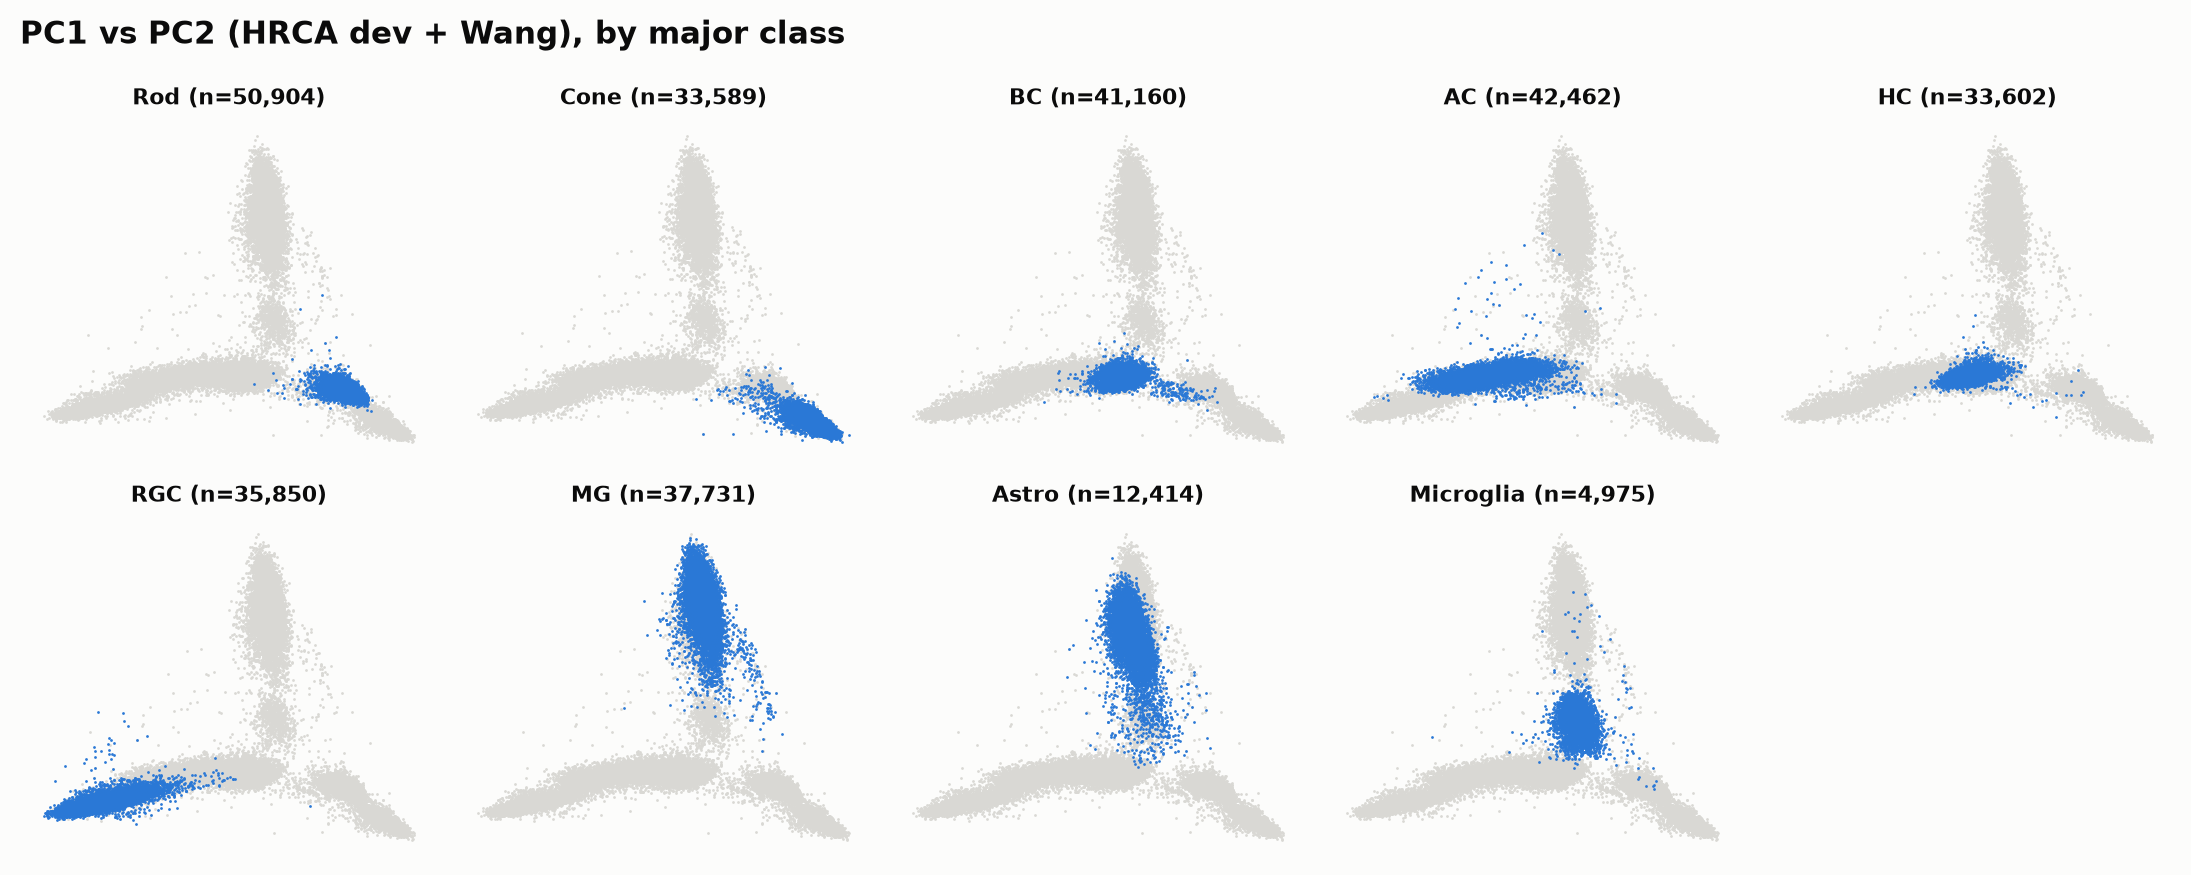
\includegraphics[width=0.93\textwidth]{eda_pca_by_class.png}\\[-1pt]
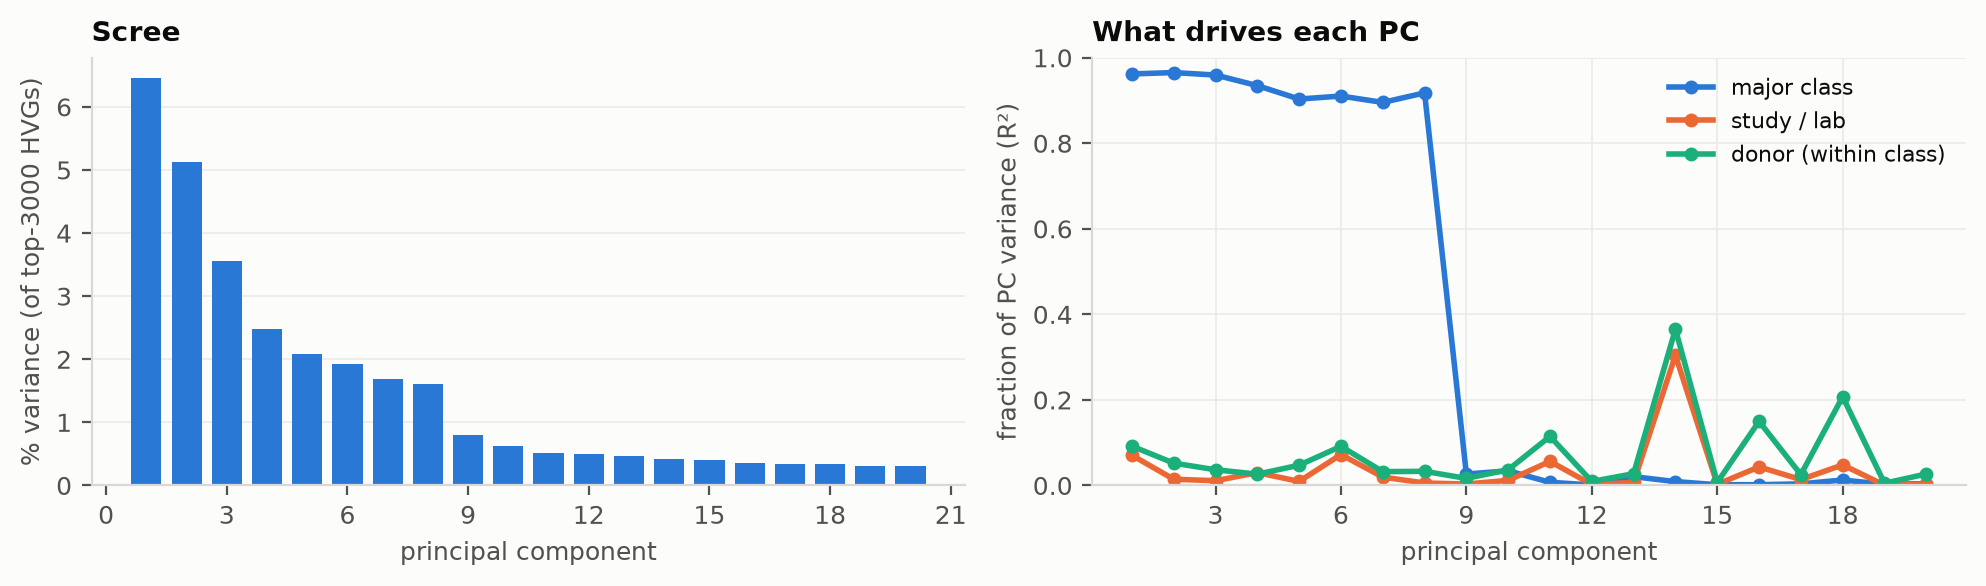
\includegraphics[width=0.78\textwidth]{eda_pca_variance.png}
\caption{\textbf{a}, PC1 vs.\ PC2 of HRCA major-task cells plus 20k Wang cells. Each panel
highlights one class. \textbf{b}, Scree plot (left) and, for each PC, the fraction of
variance explained by major class, study/lab, and donor within class (right).}
\label{fig:pca}
\end{figure}

% ---------------------------------------------------------------------------
\section{Methods}

\textbf{Evaluation protocol.} All methods use the same 5-fold donor-grouped stratified
cross-validation, so every donor's cells fall in exactly one test fold, and the code checks
this. Everything data-dependent is fit on training donors only: the HVGs, the z-score
parameters, the DE rankings and the learned panels. Inputs are
$\log(1+\mathrm{CP10k})$, z-scored and clipped at $\pm10$. For the major task we also apply
each fold's model to Wang without retraining. We also run a lab-held-out split: train on
Chen-lab donors and test on the 17 Shekhar-lab donors. The primary metric is macro
one-vs-rest auPR. We also report macro-F1 and balanced accuracy, plus 95\% CIs from
resampling donors on pooled out-of-fold predictions.

\textbf{Baselines.} (i) L2 multinomial logistic regression (LR) on all 3{,}000 HVGs.
(ii) Panels of $k\in\{10,25,50,100,200\}$ genes, all chosen from the same HVG set:
\emph{random} (3 seeds); \emph{HVG}, the top-$k$ by seurat-v3 variance rank; and \emph{DE},
from Wilcoxon one-vs-rest tests (scanpy~\cite{wolf2018}). For DE, each class's up-regulated
genes are taken round-robin, one per class at a time, until $k$ distinct genes are chosen.
Every panel is scored with the same downstream L2 LR on its $k$ genes.

\textbf{Concrete selector.} The selector has $k$ rows, and each row is a categorical
distribution over the $G$ genes, parameterized by logits $\boldsymbol\ell_j$. During training
the selected features are $\mathbf{x}^\top\mathrm{softmax}((\boldsymbol\ell_j+\mathbf{g})/T)$,
where $\mathbf{g}$ is Gumbel noise. These feed a 2-layer MLP (256 units, BatchNorm, dropout
0.2). At evaluation each row takes the argmax gene. A penalty on total selection mass above
1 for any gene discourages picking the same gene twice. The donor-adversarial variant adds a
donor classifier that sees the selected genes \emph{and} the true class, connected through
gradient reversal with $\lambda=1$ ramped up as in~\cite{ganin2016}. Conditioning on the
class means only donor signal beyond class composition is penalized. We report the panel
scored with the shared LR (\texttt{concrete}). The end-to-end MLP's scores, which we label
\texttt{concrete\_mlp} in our results files, are not shown here.

\textbf{What did not work at first.} Following~\cite{abid2019} exactly (one learning rate of
$10^{-3}$, $T$ annealed from 10 to 0.01) failed. Accuracy \emph{dropped} as $T$ fell and
ended at the majority-class rate, because the logits could not sharpen before the selection
hardened. Three changes fixed this: a separate, larger learning rate for the logits
($5\times10^{-2}$); starting at $T_0=2$ and finishing the anneal at 75\% of training, so the
head can adapt to the hard selection; and inverse-frequency class weights. We also run on
CPU, because PyTorch's Apple-GPU (MPS) backend crashed on our machine.

% ---------------------------------------------------------------------------
\section{Preliminary results}

\textbf{Major classes are close to solved within HRCA; the external test is the real
challenge.} The full LR reaches macro auPR 0.9999 on held-out donors and on the held-out
lab. A 25-gene DE panel already gets 0.996 (Fig.~\ref{fig:bench}a, Table~\ref{tab:k50}). On
Wang, the full model drops to 0.967 and small panels drop more: DE scores 0.786, 0.901 and
0.943 at $k=10$, 25 and 50. Per class, the loss is concentrated in rare glia. With $k=50$,
Wang microglia score 0.71--0.75 auPR (vs.\ 0.89 with all genes) and astrocytes 0.89, while
every neuronal class stays at or above 0.95. HVG panels at $k=50$ miss cones almost entirely
(auPR 0.51). Picking genes per class, as DE does, clearly beats picking by variance.

\begin{figure}[t]
\centering
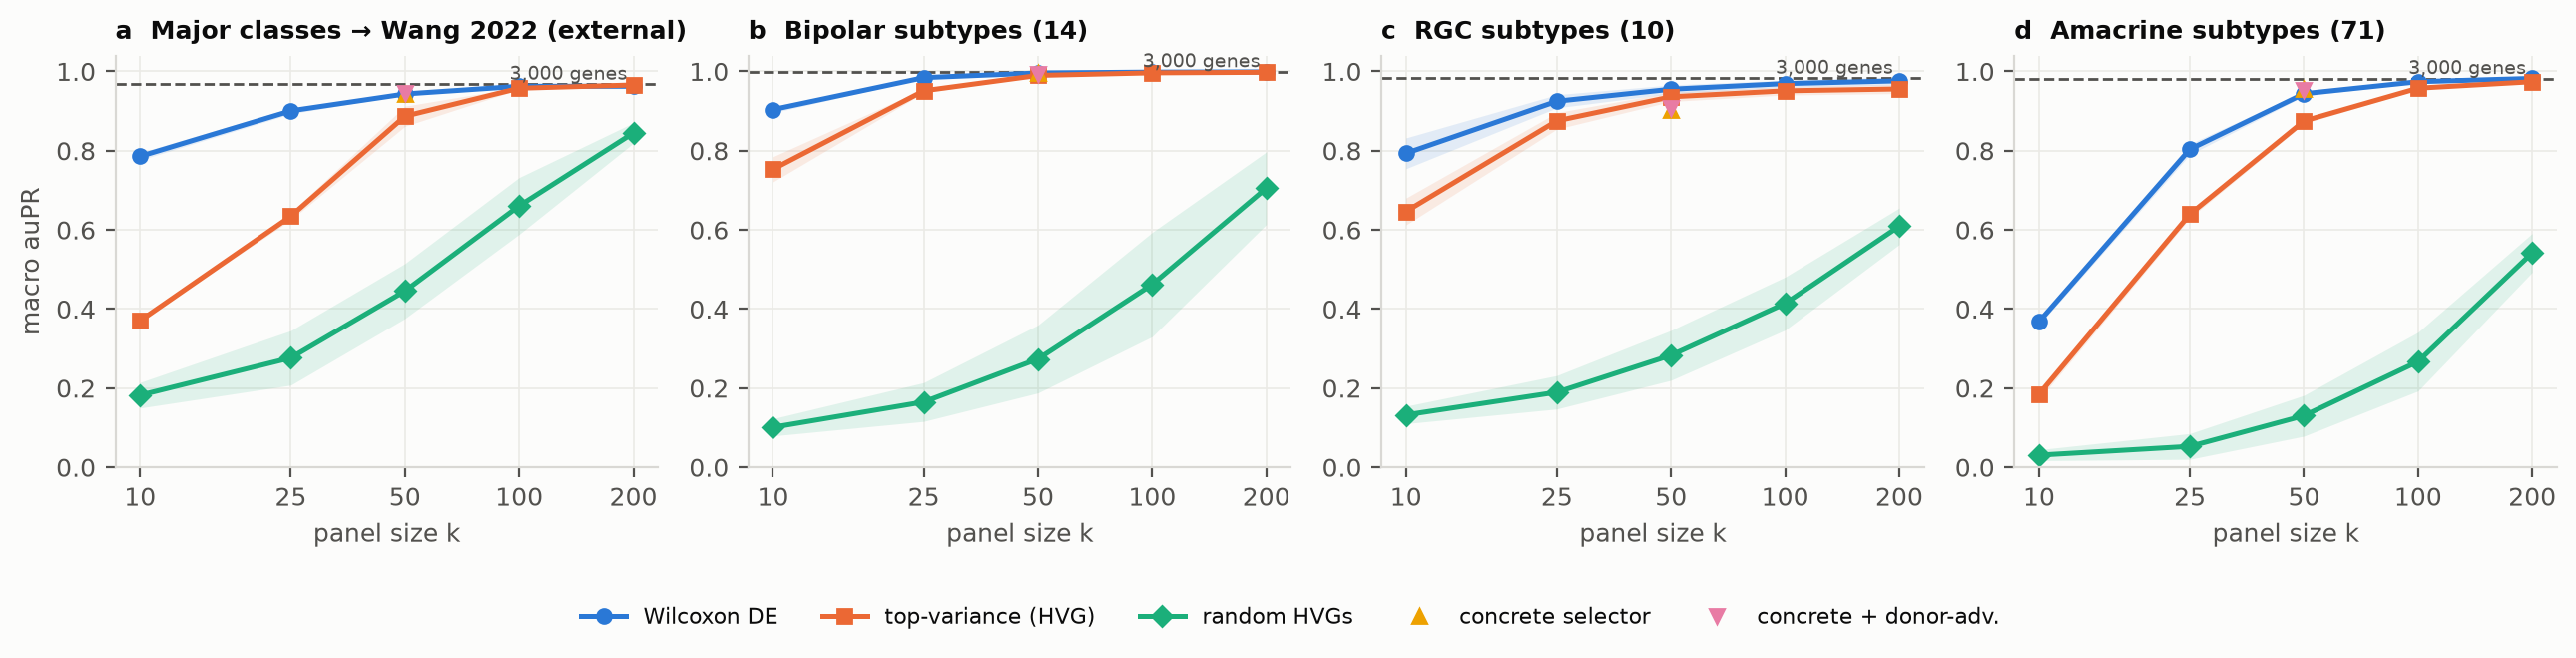
\includegraphics[width=\textwidth]{report_bench.png}
\caption{Macro auPR vs.\ panel size (mean $\pm$ s.d.\ over 5 donor folds). \textbf{a},
Major classes on Wang 2022 without retraining. \textbf{b--d}, Subtype tasks on held-out HRCA
donors. The dashed line is the 3{,}000-gene LR. Concrete selectors were run only at $k=50$.}
\label{fig:bench}
\end{figure}

\begin{table}[h]
\centering\small
\caption{Macro auPR at $k=50$ (pooled out-of-fold predictions, 95\% donor-bootstrap CI). For
Wang, values are mean $\pm$ s.d.\ over the 5 fold models. Best panel in bold.}
\label{tab:k50}
\begin{tabular}{lccccc}
\toprule
task & full LR (3000) & HVG & DE & concrete & concrete + adv. \\
\midrule
major, held-out donors & 0.9999 & 0.968 & 0.9987 & \textbf{0.9993} [.9989,.9996] & 0.998 \\
major $\to$ Wang 2022 & 0.967$\pm$.001 & 0.887$\pm$.025 & 0.943$\pm$.002 & 0.944$\pm$.005 & \textbf{0.946}$\pm$.005 \\
BC subtypes (14) & 0.999 & 0.990 & 0.996 [.995,.997] & \textbf{0.997} [.996,.997] & 0.995 \\
RGC subtypes (10) & 0.982 & 0.935 & \textbf{0.954} [.945,.961] & 0.905 [.891,.917] & 0.906 \\
AC subtypes (71) & 0.981 & 0.874 & 0.944 [.937,.949] & \textbf{0.955} [.950,.960] & 0.953 \\
\bottomrule
\end{tabular}
\end{table}

\textbf{Subtypes separate the methods, and DE is a strong baseline.} As the course feedback
predicted, the learned selector only modestly beats DE, and not on every task
(Table~\ref{tab:k50}). On BC subtypes the two are tied within the CIs (0.997 vs.\ 0.996). On
AC subtypes the concrete selector wins clearly (0.955 vs.\ 0.944, non-overlapping CIs).
There, round-robin DE allots fewer than one gene to each of the 71 classes, while a learned
panel can use genes that separate several subtypes at once. On RGC subtypes the concrete
selector \emph{loses} (0.905 vs.\ 0.954). This task has the least training data (about
16k cells per fold), and 95\% of RGCs in the atlas are midget cells, which hurts the
selector's balanced training. Random panels are poor everywhere (0.13--0.68 at $k=50$),
which confirms that gene choice matters.

\textbf{The donor-adversarial head does not help yet.} With $\lambda=1$, held-out
performance is the same or slightly lower on every task, and the gain on Wang (0.946 vs.\
0.944) is within the fold-to-fold noise. Its donor classifier reaches only about 5\% accuracy (chance is
1.2\%). So even without the penalty, the selected genes carry little donor information
beyond class, which matches the PCA analysis.

\textbf{Learned panels are less stable.} Across the five folds at $k=50$, DE panels are
nearly the same (mean pairwise Jaccard index 0.90), but concrete panels are not (0.44, and
0.25 with the adversary). In fold~0, 21 of the 50 concrete genes are also in the DE panel,
including canonical markers such as \emph{SAG} and \emph{ABCA4} (photoreceptors),
\emph{PTPRC} (microglia) and \emph{CRB1} and \emph{ATP1A2} (MG). The concrete panel also
picks \emph{GAD1} (GABAergic AC), which the DE panel does not. The low overlap suggests that many different gene sets work about equally well.

\textbf{ATAC preprocessing.} For each of the 13 Wang ATAC cell types we counted Tn5
insertions within $\pm2$\,kb of each TSS (and over gene body + promoter), then normalized
to counts per million. Known markers are most accessible in the expected cell type:
\emph{ARR3} and \emph{PDE6H} in cones, \emph{GRM6} in ON-cone BCs, \emph{POU4F2} in RGCs,
\emph{RLBP1} in MG, \emph{GFAP} in astrocytes, and \emph{PTPRC} and \emph{C1QA} in microglia.
Some markers are not, for example \emph{PRKCA} (rod BC) and \emph{RBPMS} (RGC). This
supports the course feedback: promoter accessibility is an imperfect and generic readout,
so the right comparison is learned panels vs.\ DE panels of the same size.

% ---------------------------------------------------------------------------
\section{Next steps}

\begin{itemize}
\item \textbf{Run the selector at every panel size, with repeats.} We will run concrete
selection at all $k$ and over several seeds. To tackle panel instability, we will pick a
consensus panel by selection frequency across folds and seeds.
\item \textbf{Improve the selector where it loses.} For RGC subtypes, initializing the
selector from DE rankings and training longer may help, so the learned method starts at
least as well as DE. We will also add PERSIST~\cite{covert2023} and group-lasso LR as
learned baselines.
\item \textbf{Retest the donor-adversarial head where donor effects are larger.} We will
sweep $\lambda$ and apply it on the lab-held-out split, where the gap is bigger. If it still
does not help, we will report that negative result.
\item \textbf{Pretrained comparisons.} We will add frozen TranscriptFormer embeddings with
an LR probe. We still need to check whether Pan-human Azimuth's retinal labels can be mapped
to our classes; this was an interim goal we have not completed.
\item \textbf{ATAC validation as suggested.} For each cell type, we will compare the
promoter accessibility specificity of learned-panel genes with DE-panel genes of the same
size and with expression-matched random genes, using permutation tests. We will also measure
marker overlap (precision@$k$) against published retinal markers.
\item \textbf{Pitfalls.} Wang has only 4 donors and 231 microglia, so its per-class CIs will
be wide. We will report per-class results and donor-bootstrap intervals. The lab-held-out
split has a single test lab, so there is no fold-to-fold spread to report for it.
\end{itemize}

\textbf{Questions.} Should the external evaluation keep or merge rare glial classes, given
how few Wang cells they have? Is initializing the selector from DE genes acceptable, or does
it blur the comparison with the DE baseline?

\printbibliography
\end{document}
